\section{ХОД РАБОТЫ}

\subsection{Постановка задачи}

При помощи технологии WCF создайте распределенное приложение-чат,
которое включает в себя две составляющие: службу и клиента.

Служба должна выполнять следующие функции:
\begin{itemize}
\item добавление сообщения;
\item получение сообщений.
\end{itemize}

В качестве хранилища сообщений должна использоваться база данных.
В качестве хоста для службы можно выбрать консольное приложение.
В качестве приложения-клиента должно выступать оконное приложение.

В приложении-клиенте должен быть реализован просмотр сообщений,
добавление сообщений, а также получение сообщений.

Для каждого сообщения должен отображаться текст сообщения, имя
автора, а также дата добавления.

При запуске приложение-клиент должно запрашивать имя пользователя и
адрес службы, без ввода которых приложение не должно позволять выполнять
какие-либо действия.

Получение сообщений должно быть реализовано следующим образом:
если приложение-клиент еще не загружало сообщения, то оно должно
запрашивать у службы все сообщения, имеющиеся в базе, иначе должны быть
загружены только те сообщения, которые были добавлены после последнего
запроса списка сообщений.

\subsection{Особенности разработанного приложения}

Неформально взаимодействие между клиентом и сервером можно описать следующим образом.

Клиент периодически запрашивает сервер на предмет наличия новых сообщений.
Сообщение считается новым, если оно было сохранено в базе данных позже,
чем указано в параметре запроса.
Сервер проверяет содержимое своей базы данных и формирует список новых сообщений,
затем передаёт его клиенту.

Кроме этого, клиент может выполнять отправку нового сообщения на сервер.
В этом случае сервер выполняет сохранение этого сообщения в базе данных.

Протокол взаимодействия приложения-клиента с приложением-сервером определяется контрактом,
приведенным на рисунке~\ref{lst:service_contract}.

\begin{lstlisting}[caption=Контракт взаимодействия клиента с сервером,
label=lst:service_contract,language={Java},basicstyle=\scriptsize\ttfamily]
[ServiceContract]
public interface IMsgService
{
  [FaultContract(typeof(FaultException))]
  [OperationContract]
  bool checkConnection();

  [FaultContract(typeof(FaultException))]
  [OperationContract]
  List<Message> getMessages(DateTime fromDate);

  [FaultContract(typeof(FaultException))]
  [OperationContract]
  void sendMessage(Message msg);
}    
\end{lstlisting}

В данном контракте определены три функции:
\begin{itemize}
\item \texttt{checkConnection} --- выполняет проверку соединения между клиентом и сервером;
\item \texttt{getMessages} --- получает список сообщений с указанного момента времени;
\item \texttt{sendMessage} --- посылает сообщение на сервер.
\end{itemize}

Сообщение представляет собой экземпляр класса \texttt{Message}, 
представленного на рисунке~\ref{lst:message}.

\begin{lstlisting}[caption=Класс \texttt{Message},
label=lst:message,language={Java},basicstyle=\scriptsize\ttfamily]
public class Message
{
  public String Sender { get; set; }

  public String Content { get; set; }
  
  public DateTime Timestamp { get; set; }
  
  public Message(String Sender, String Content, DateTime Timestamp)
  {
    this.Sender = Sender;
    this.Content = Content;
    this.Timestamp = Timestamp;
  }
}
\end{lstlisting}

Использование методов, инкапсулирующих поля класса \texttt{Message},
позволяет прозрачно изменять внутреннюю реализацию без
затрагивания кода, использующего данный класс.

В качестве СУБД, выполняющей хранение сообщений, используется \texttt{sqlite}.

На рисунке~\ref{pic:interface} приведен пользовательский интерфейс
разработанного приложения-клиента.

\begin{figure}[h!]
  \centering
  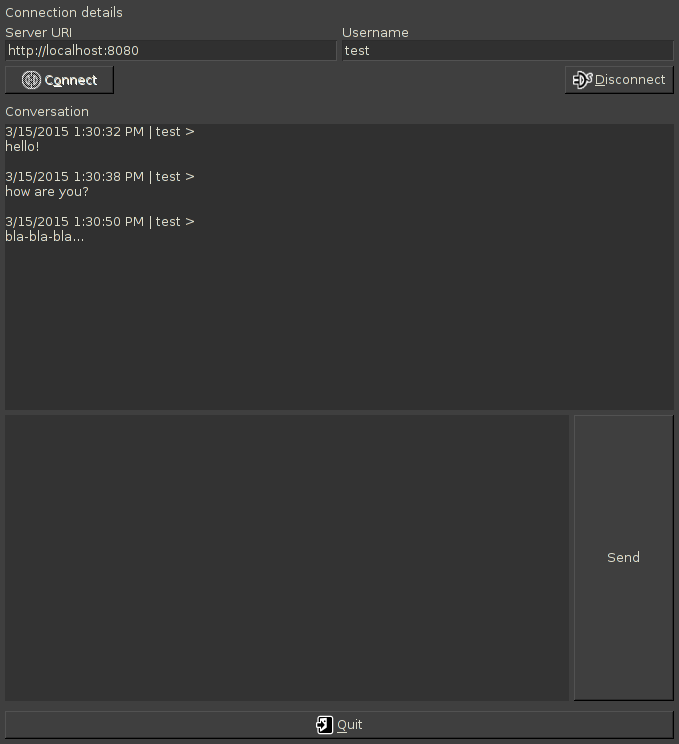
\includegraphics[width=150mm]{pic/interface}
  \caption{Интерфейс разработанного приложения}
  \label{pic:interface}
\end{figure}

Исходный текст разработанного приложения находится в приложении~А.